\documentclass{article}
\usepackage[utf8]{inputenc}
\usepackage{amsmath}
\usepackage{amssymb}
\usepackage{graphicx}
\usepackage[english]{babel}
\usepackage{amsfonts}
\usepackage{fancyvrb}
\usepackage{xcolor}
\usepackage{listings}
\usepackage{graphicx}
\usepackage{mathrsfs}
\usepackage[margin=60pt, footskip=20pt]{geometry}
\definecolor{MyDarkGreen}{rgb}{0.0,0.4,0.08}
\usepackage{tabularx}
\usepackage{blindtext}
\usepackage{wrapfig}

\usepackage{siunitx}

\begin{document}
	
\pagenumbering{gobble}
\vspace*{-1.5cm}{
	\begin{center}
		\large
		POLITECNICO DI MILANO\\
		\normalsize
		Master Degree in Mathematical Engineering\\
		Industrial and Information Engineering\\
		Department of Mathematics\\
		\begin{figure}[htbp]
			\begin{center}
				
\includegraphics[width=3.5cm]{polimi.jpg}
			\end{center}
		\end{figure}
		\vspace*{0.3cm} \LARGE
		
		
		
		\textbf{Air Quality forecasting}\\
		
		
		\vspace*{.75truecm}\large
		\vspace*{.5truecm} \large
		 Bayesian Statistics Project Report
	\end{center}
	\vspace*{3.0cm} \large

	\begin{flushright}
		
		
		Group members:\\
		Datena Amedeo \\
		Dell'Atti Martina \\
		Palummo Alessandro
		
		
	\end{flushright}
	\vspace*{2.0cm}
	\begin{center}
		
		
		
		Academic Year 2020-2021
	\end{center} \clearpage
}

\section{Wiseair and data measurement}

\subsection{Wiseair}

The measure of air quality in Lombardy is carried out by ARPA using accurate sensing stations. These stations, however,
 are expensive and bulky, so only a few of them are deployed on the territory. Only two of these stations are present in Milan. 


However, the stations only measure the air quality of their immidiate surroundings, and air quality  can be different in each neighborhood
 of the city. Air quality is assessed by measuring the Particulate Matter (PM) concentration, and PM concentrations can vary at a hyperlocal scale.

Wiseair is a startup company that has designed a low-cost sensor, meant to be user-friendly and easy to install: Arianna.
 More than 100 citizens preordered one, and 50 of these sensors have been distributed as of July 2020, thanks to the involvement of citizens.

 Below is a map of Milan with the locations of installed and functioning Ariannas.

\begin{figure}[h!]
  \centering
  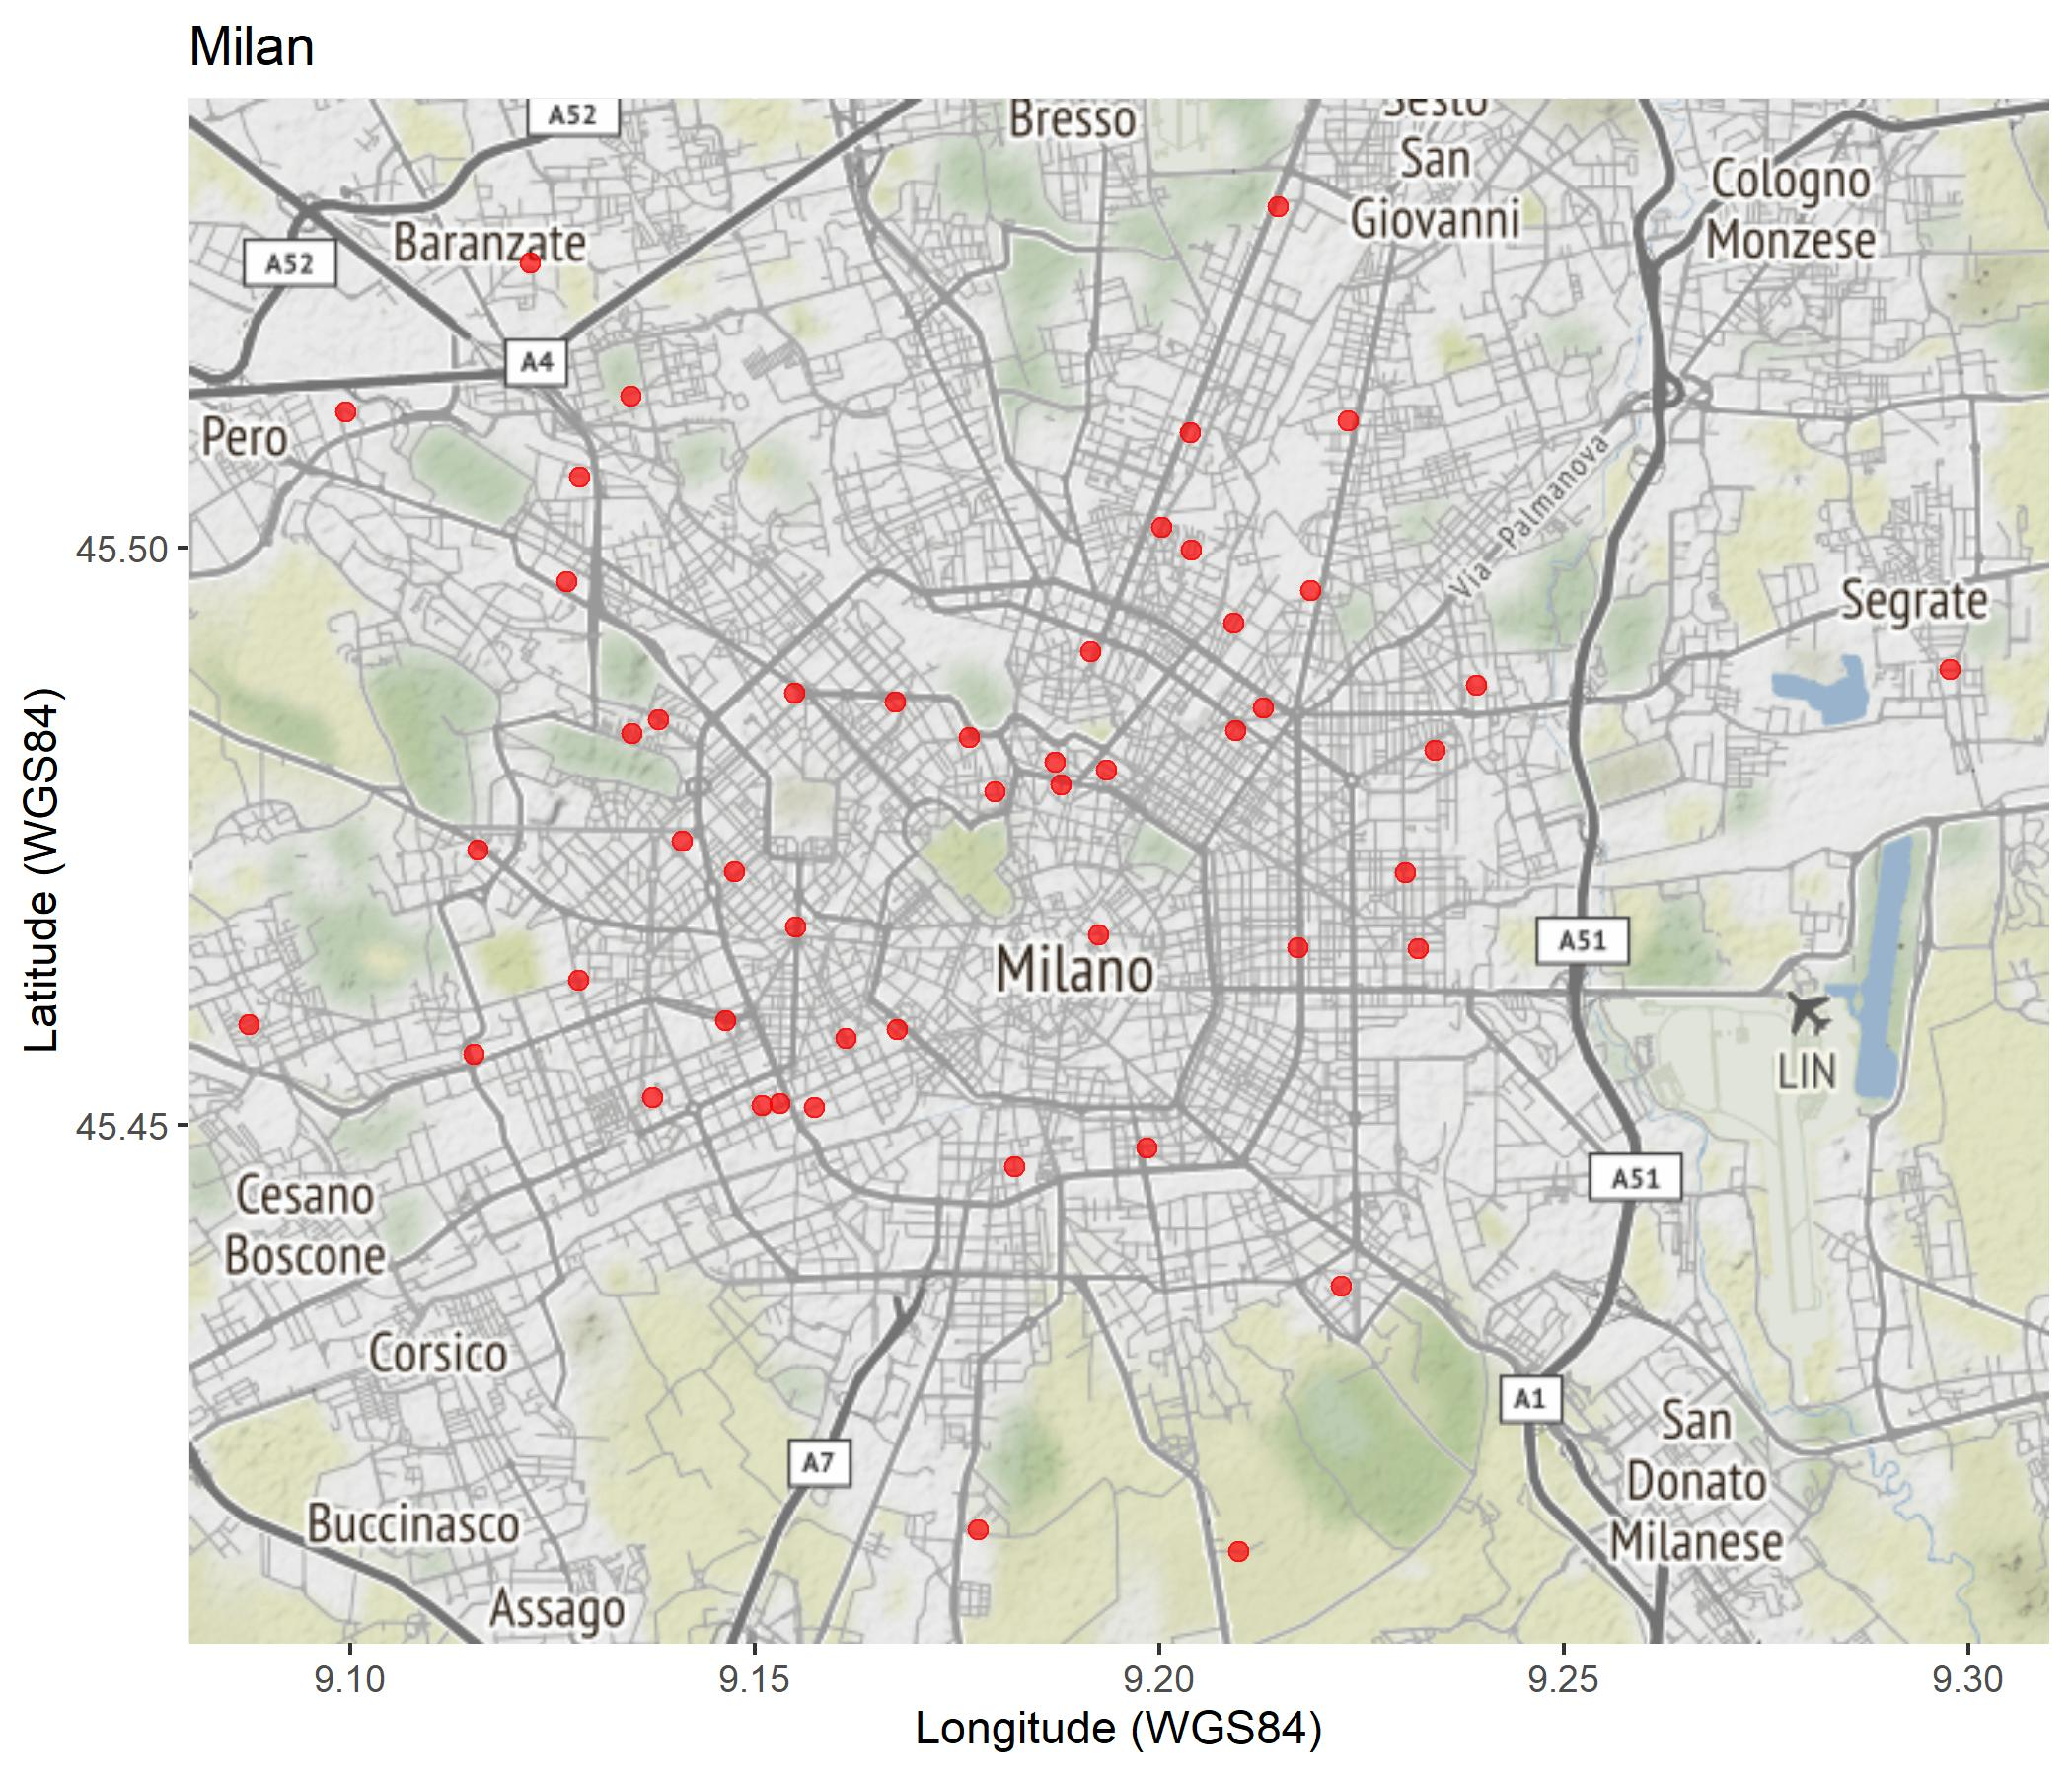
\includegraphics[width=5in]{potsMap.jpg}
  \caption{locations of installed Ariannas in the city of Milan}
\end{figure}

\subsection{Objective}

Wiseair's goal is to provide more detailed information about air quality in populated areas, so that citizens can plan outdoor activities and travel routes 
accourdingly. The first step for achieving this is a capillar measurement network in the city. The second step is the processing of data coming from the sensor
to produce information which is easily accessible for the users. 


\subsection{Data measurement}

An Arianna sensor measures the concentration of PM once per hour or more frequently. The sensor also measures humidity and 
temperature with each PM measurement. It has been observed that the measurement accuracy is negatively affected by adverse weather
 conditions, so raw data can be filtered and processed so that outliers can be detected and removed, also using humidity and temperature information.

\section{Database structure}

Each observation in the dataset is a measurement from and Arianna station. 
\begin{itemize}
    \item  The variable "PotID" identifies which sensor has taken the measurement. The ID is useful to geolocalize the measurement.
    \item The variable "created\_at" gives the time coordinate for the measurement, up to the second. The format is "yyyy-mm-dd hh:MM:ss".
    \item There are 4 variables related to air quality measurement, one for each of the following particulate matter types:
    PM\textsubscript{1},PM\textsubscript{2.5},PM\textsubscript{10}. These types refer to the thickness of the measured
    particulate (for example, the variable PM\textsubscript{2.5} refers to particles of less than 2.5 \si{\micro\meter}. The
    PM concentrations are measured in \si{\micro\gram\per\cubic\meter}.
    \item The variables "temperature" and "humidity" record the temperature and humidity measurements made by the Arianna station.
\end{itemize}

\subsection{Time irregularity}

The measurement frequency of the Arianna station can be set by the user and the stations do not transmit their measurement if
an internet connection is not
available. This means (1) that the measurement frequency varies among stations and (2) most stations do not perform measurement
at a regular time frequency:
for example, many stations stop transmitting data at night. This introduces time irregularity in the time series.
Another issue is that different stations have been installed at different times: the time series for each Arianna starts at
a different time. Below is a plot where the time irregularity is shown.

\begin{figure}[h!]
  \centering
  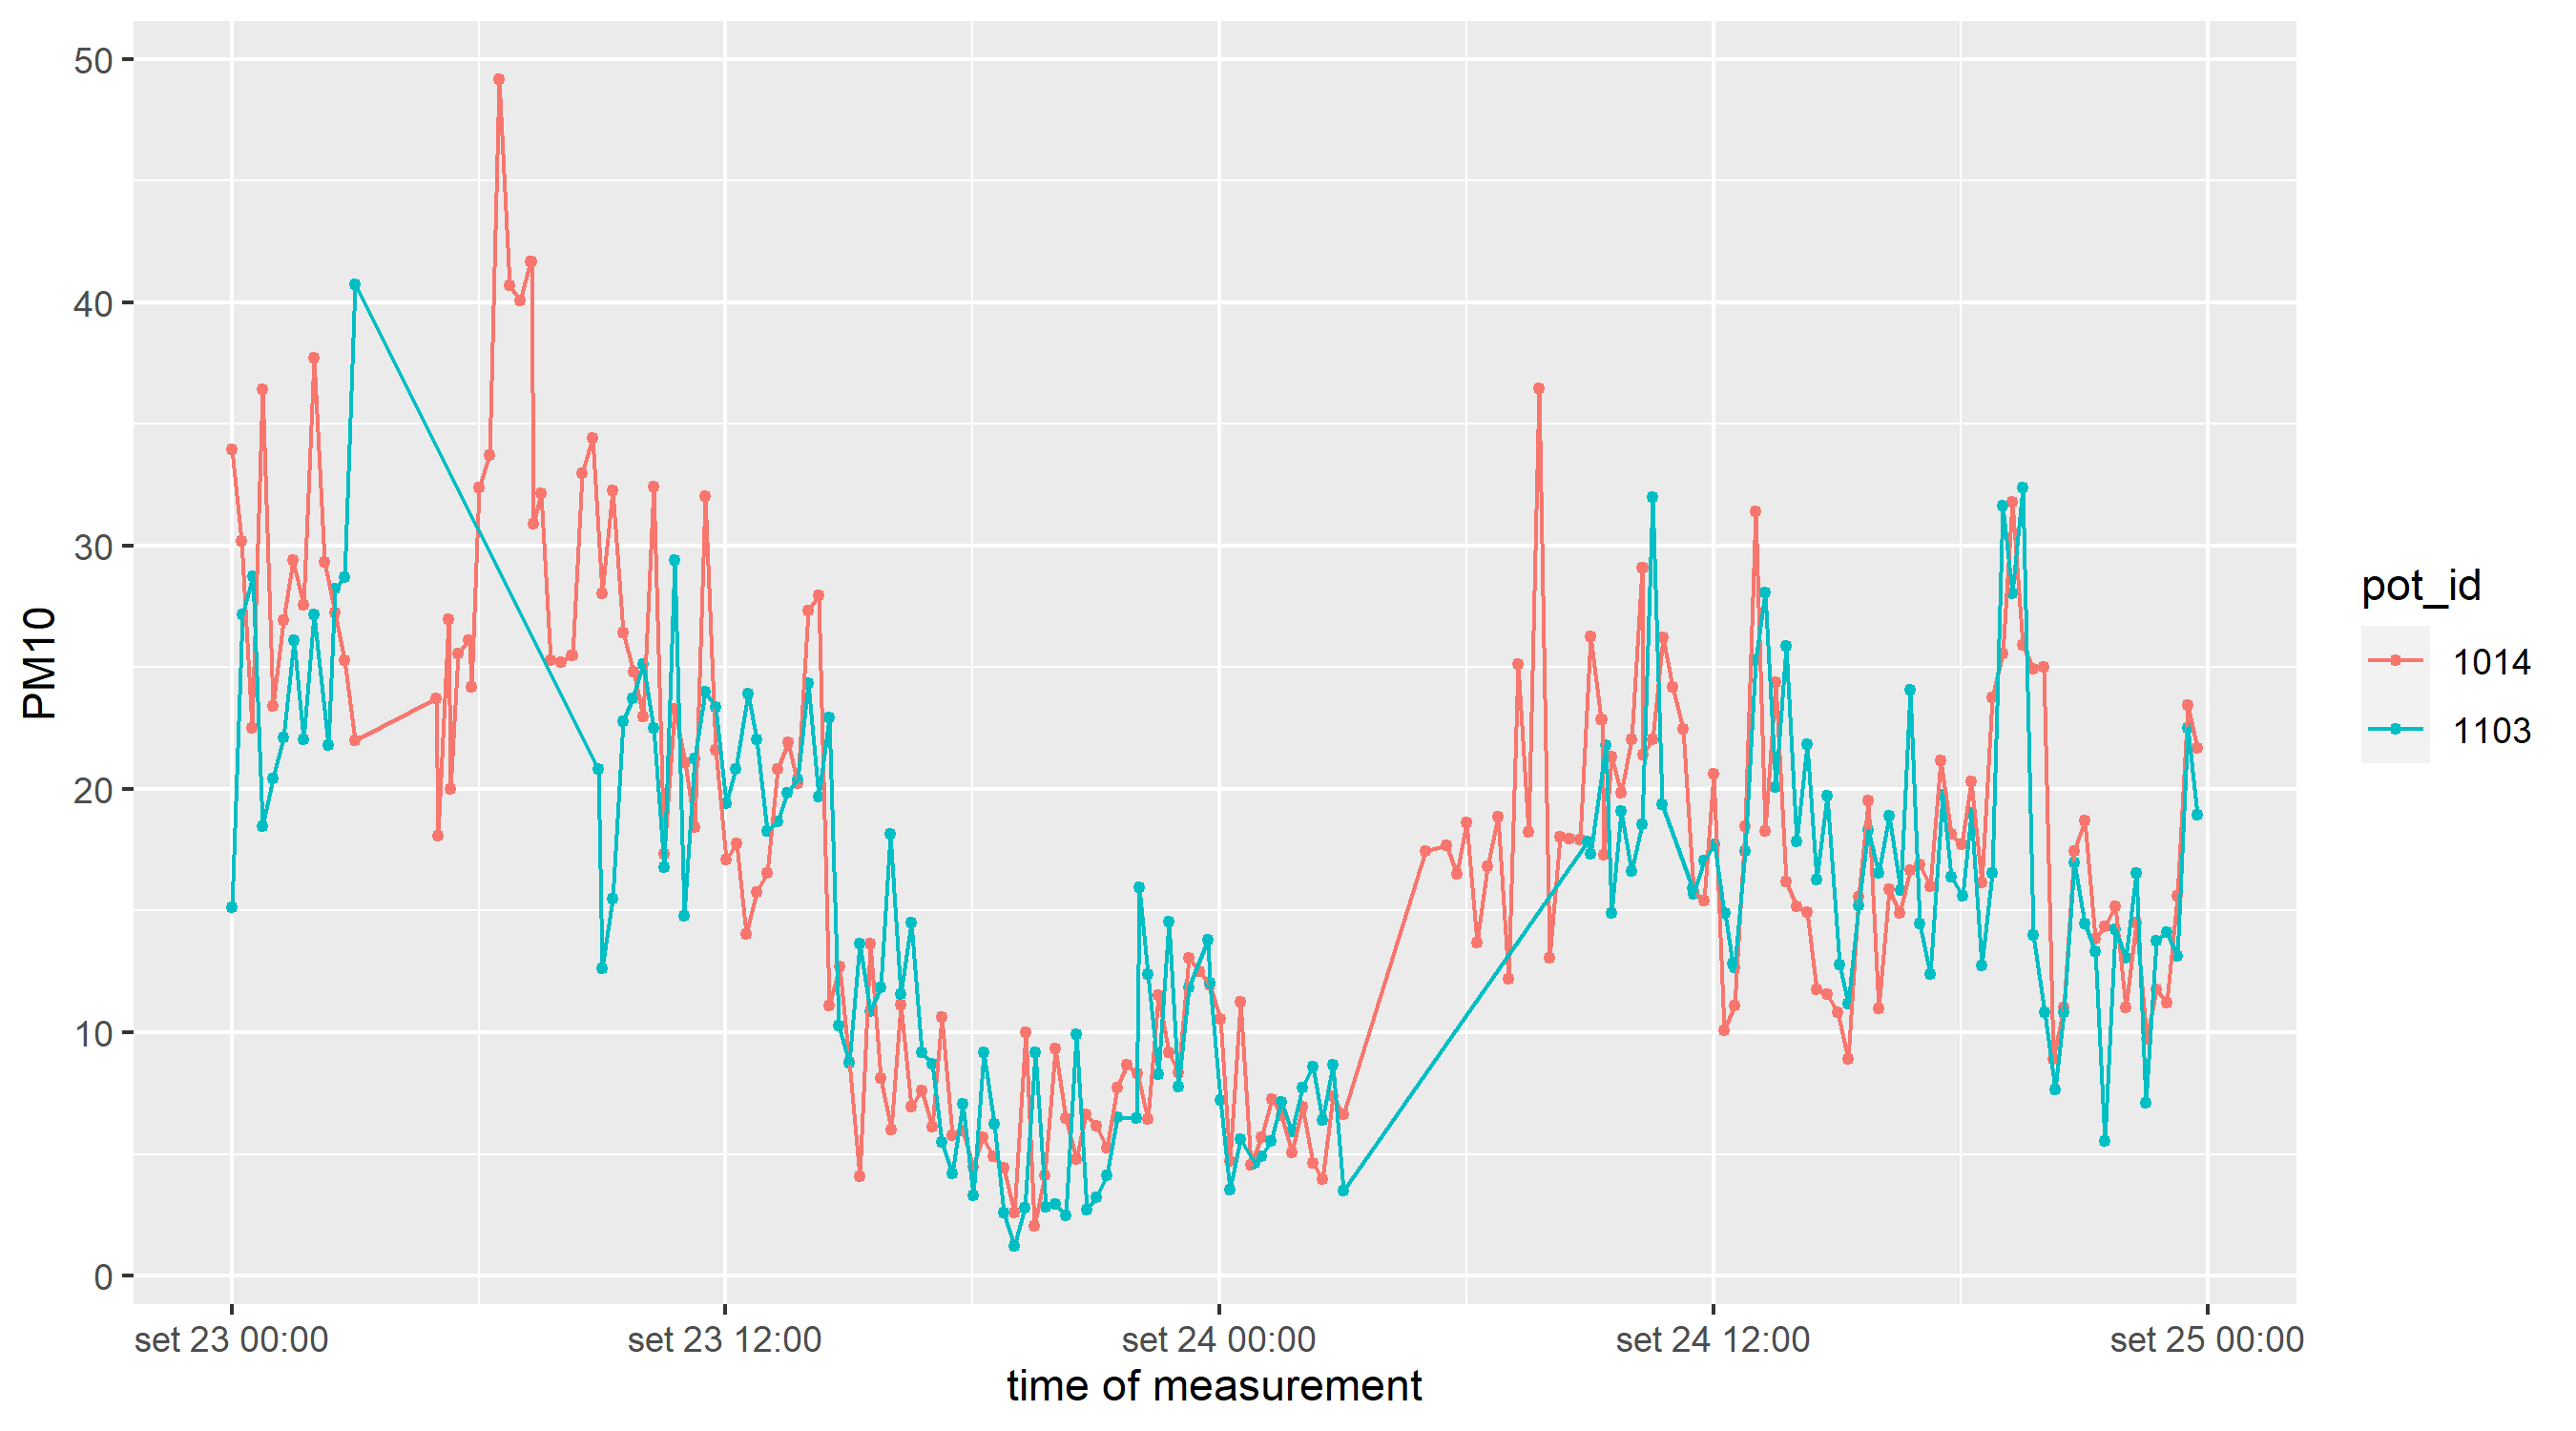
\includegraphics[width=5in]{timeIrregularity.png}
  \caption{portion of PM\textsubscript{10} measurement from two Arianna stations}
\end{figure}

Time irregularity is an issue to be solved before performing univariate or multivariate analyses, and each type of analysis might require a different approach to the issue.

Time irregularity can be solved in multiple methods. The data could be smoothed using spline curves, producing continuous
functions that can be sampled at regular time intervals. 

------
Originally we had data with a non regular frequency, i.e. the frequency of measurements of a sensor 
is different from others. For example, some pot-id make two measurements for hour, other pot-id make 
five measurements for hour. So we have performed an hourly average of the measured quantities in order to have equally spaced points. We choose to aggregate hourly because of two reasons: 
\begin{itemize}
\item This choice does not remove eventual patterns during the day, differently from the case in which we tried to aggregate taking daily averages. 
\item Weather data (rain level, wind speed) from ARPA are available with hourly frequency so we needed to average 
available data hourly before integrating further information from ARPA sensors. 
\end{itemize}

\begin{figure}[h!]
  \centering
  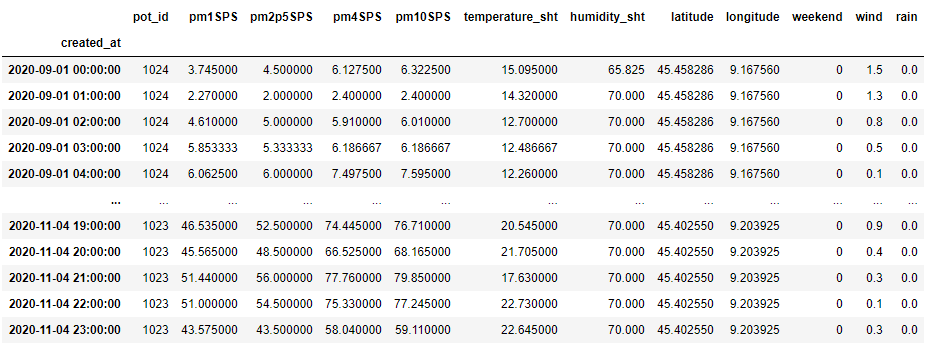
\includegraphics[width=5in]{dataset.png}
  \caption{Portion of the processed dataset}
\end{figure}


------
\newpage
\section{\textbf{Univariate Analysis}}
\subsection{Exploration analysis}
\begin{figure}[h!]
    \centering
    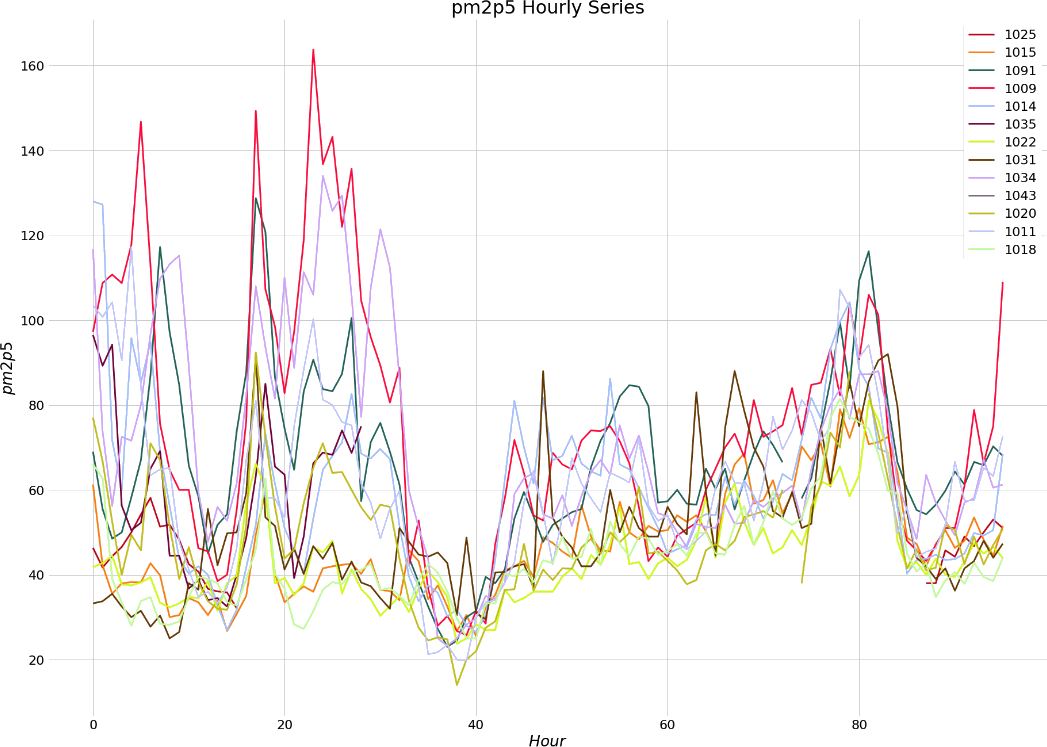
\includegraphics[scale=0.3]{plotDati.png}
    \caption{time series of pm2p5 in 48 hours for some pot-id}
\end{figure}
Wiseair own more than 60 air quality sensor in Milan at the moment and they are increasing day by day thanks to the involvement of citizens who install them.\\ 

In our dataset they are identified by the variable potid. 
We consider only one potid to make some initial exploration, in particular we consider the \textbf{potid 1091} because it is the pot with less missing values.

 \begin{figure}[h!]
    \centering
    \begin{minipage}[t]{0.4\textwidth}
      \centering
      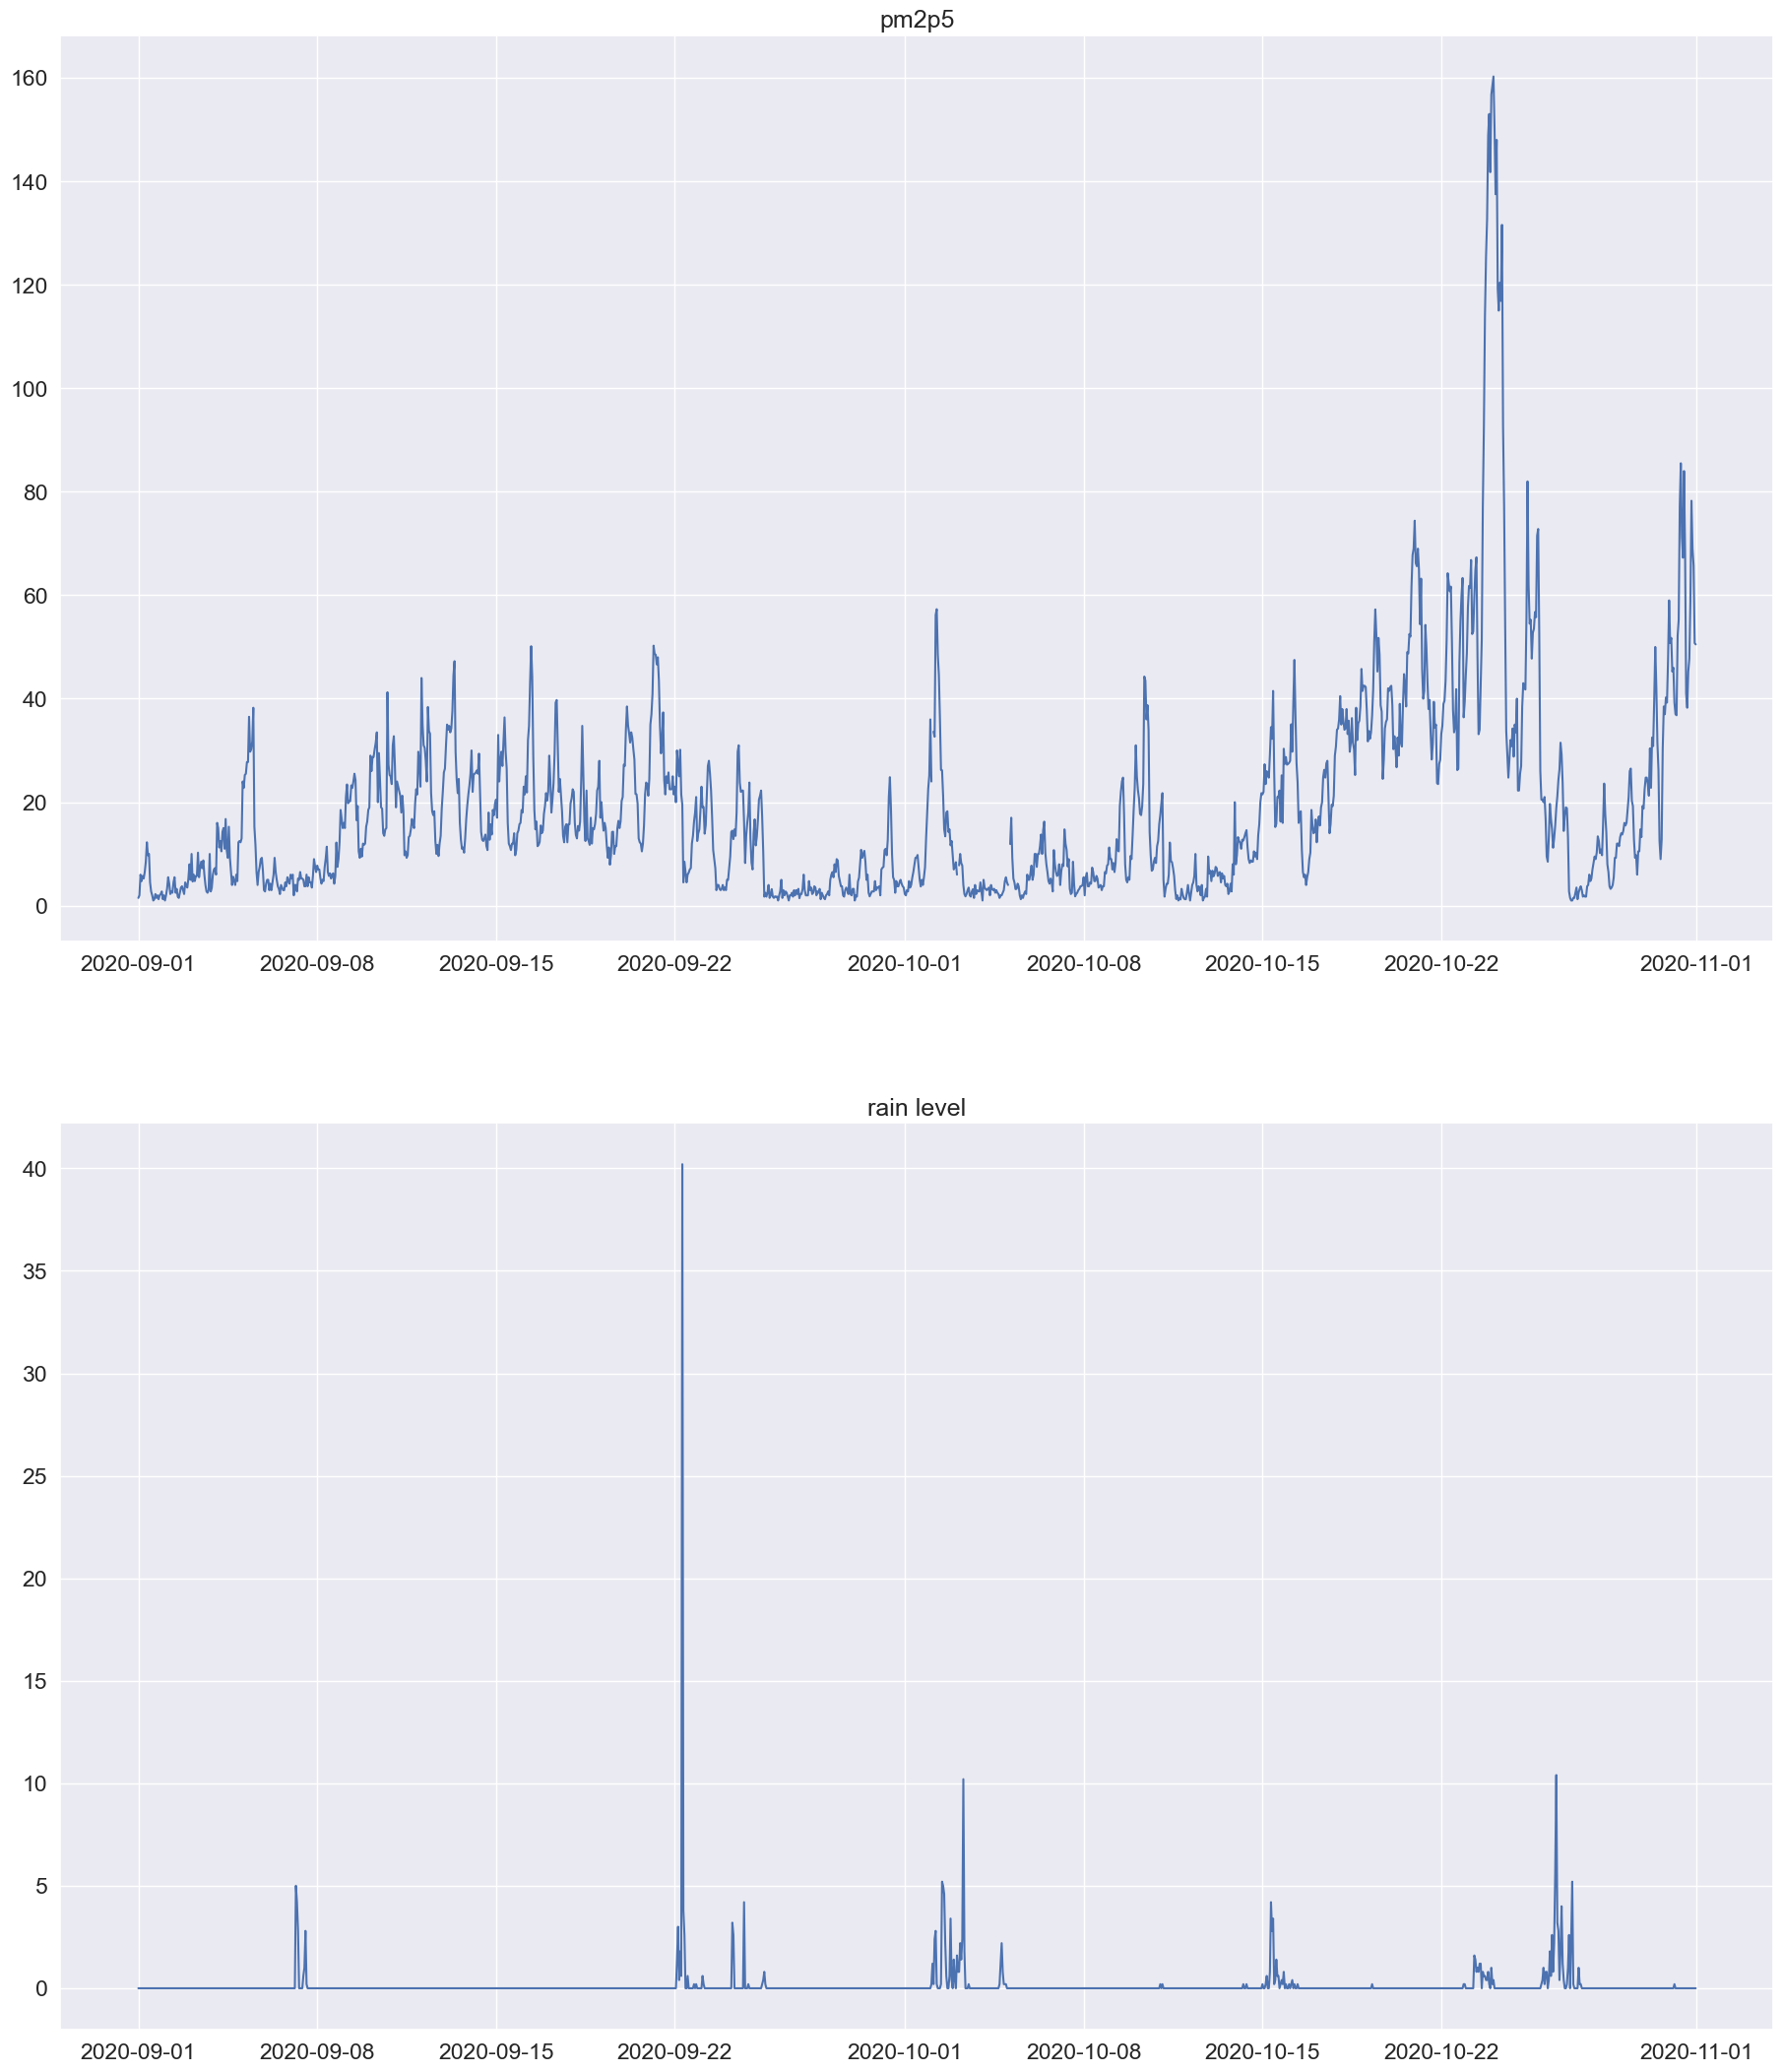
\includegraphics[scale=0.18]{plotpioggia.png}
      \caption{(a) Plot of rain vs pm2p5}
    \end{minipage}\hfill
    \begin{minipage}[t]{0.4\textwidth}
      \centering
      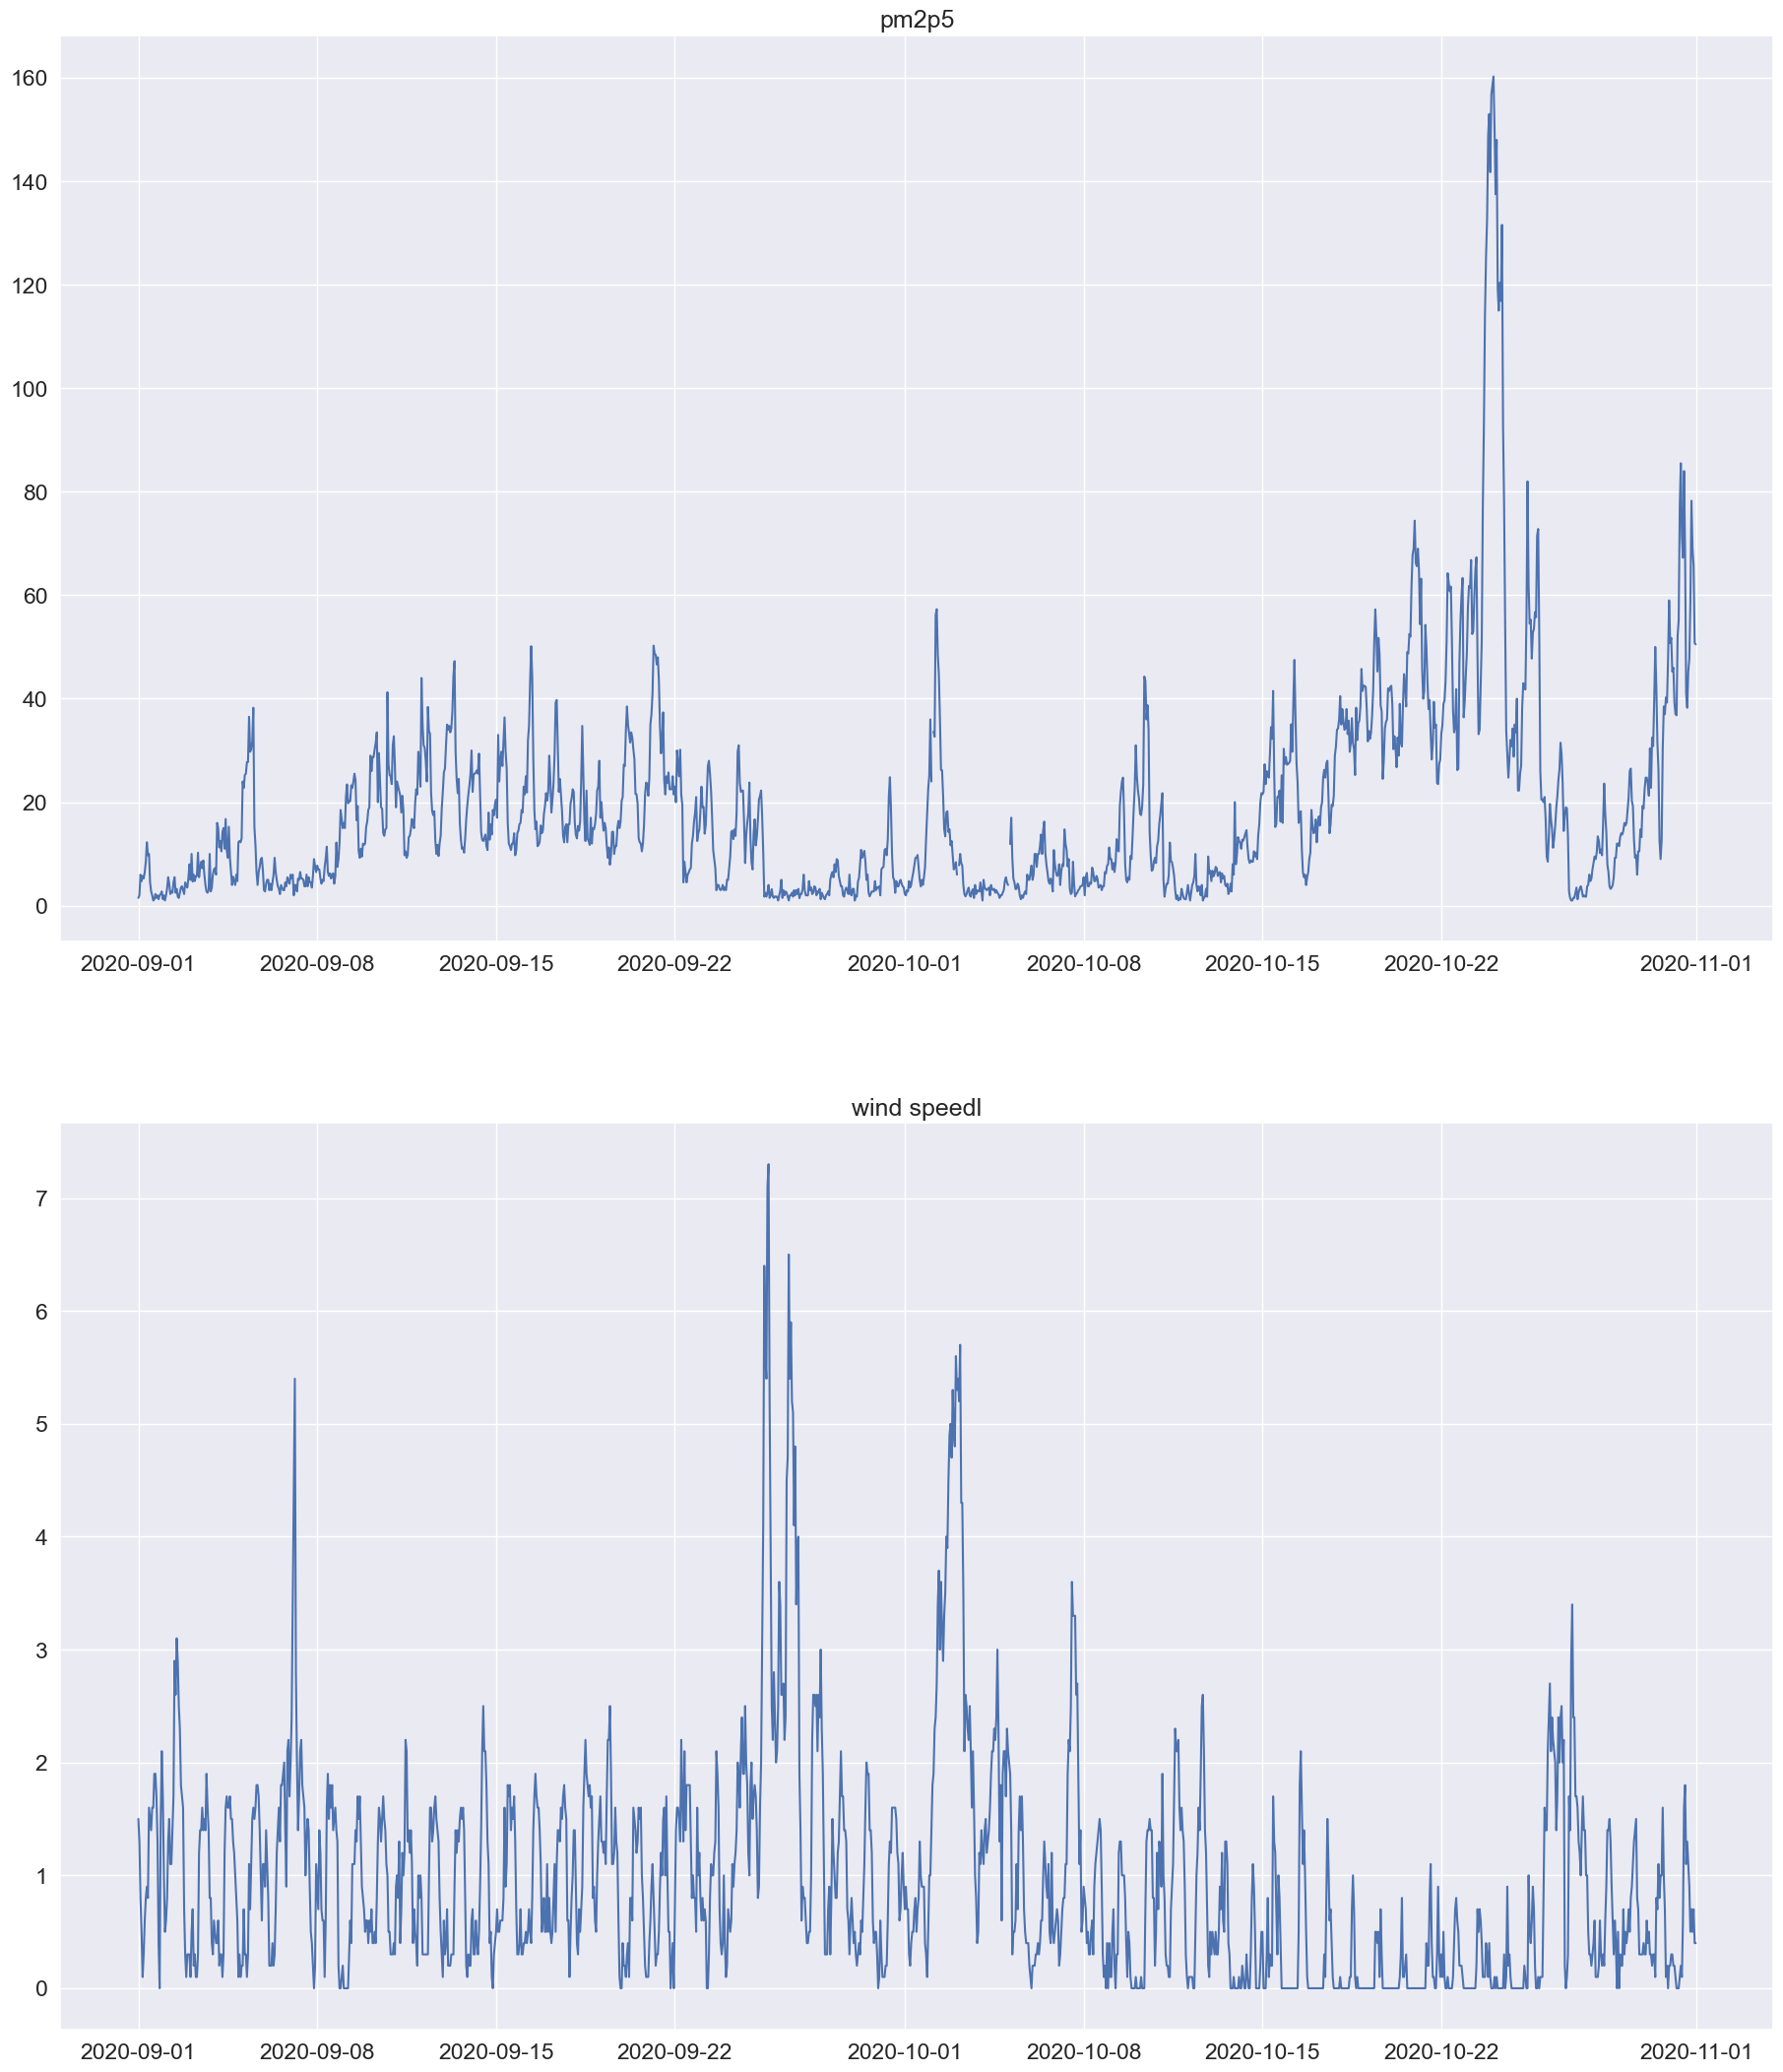
\includegraphics[scale=0.18]{plotwind.png}
      \caption{(b) Plot of wind speed vs pm2p5 }
    \end{minipage}
  \end{figure}
  
  \begin{figure}[h!]
    \centering
    \begin{minipage}[t]{0.4\textwidth}
      \centering
      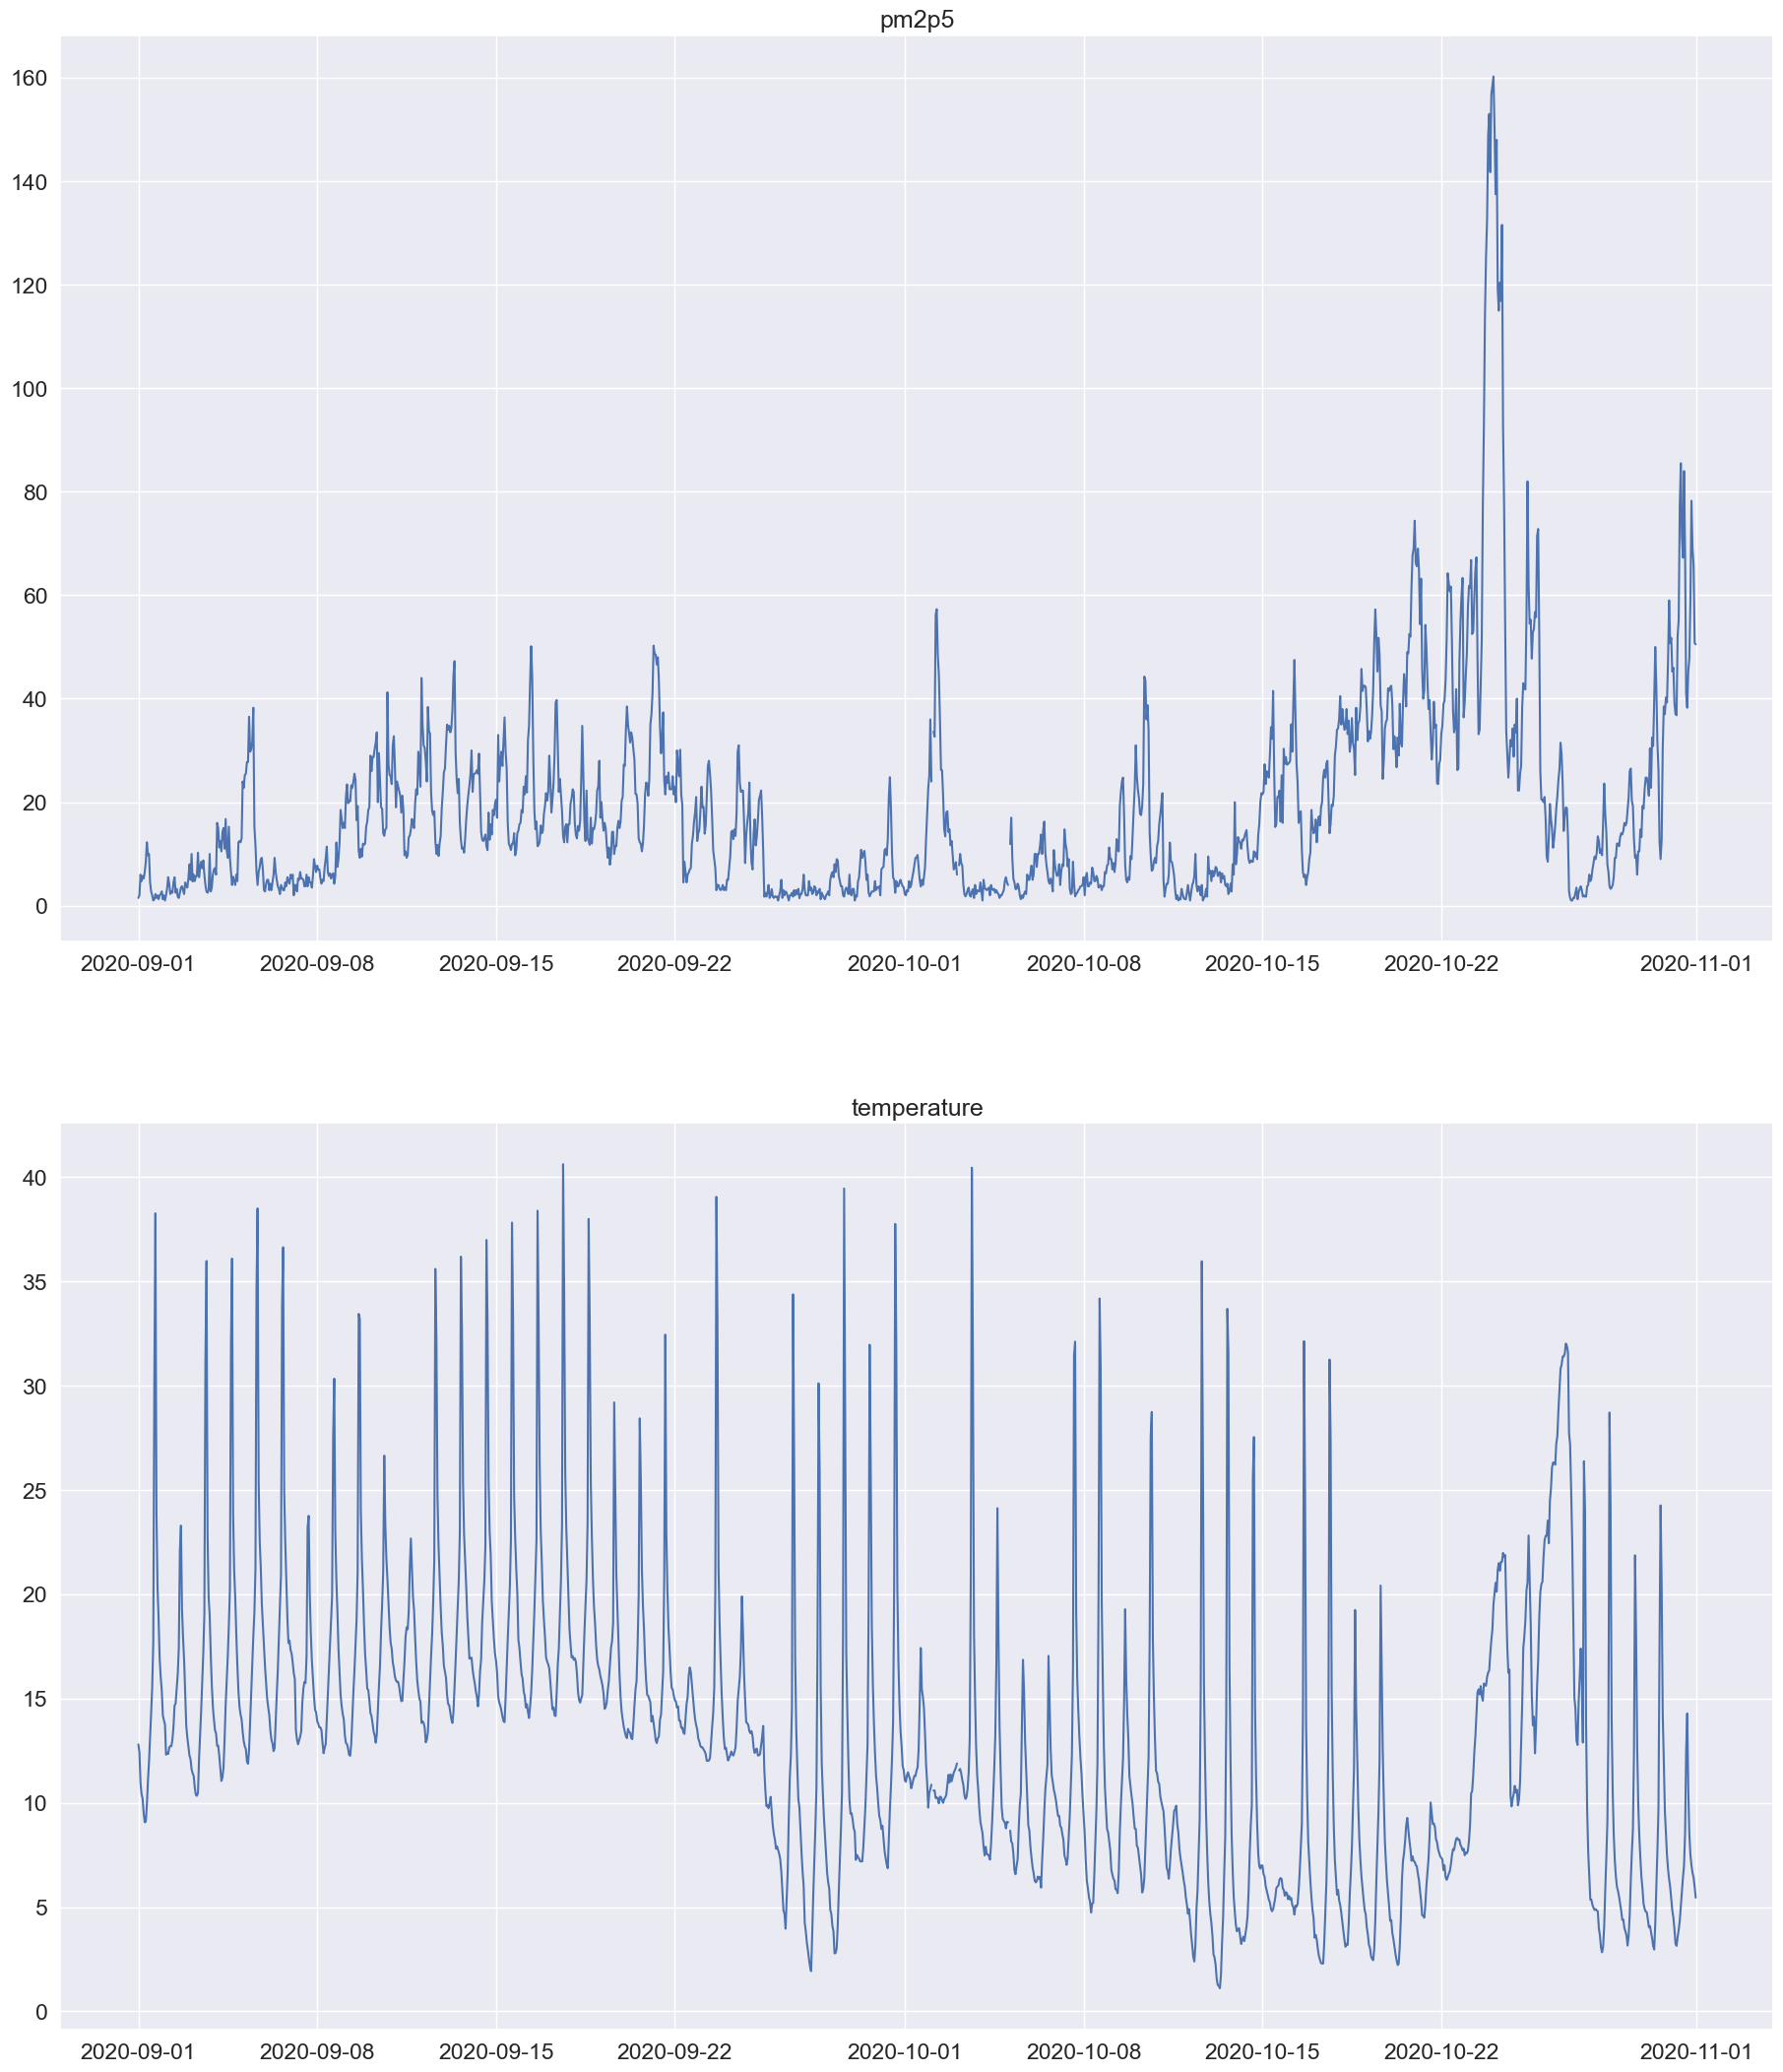
\includegraphics[scale=0.18]{plottemperature.png}
      \caption{(c) Plot of temperature vs pm2p5}
    \end{minipage}\hfill
    \begin{minipage}[t]{0.4\textwidth}
      \centering
      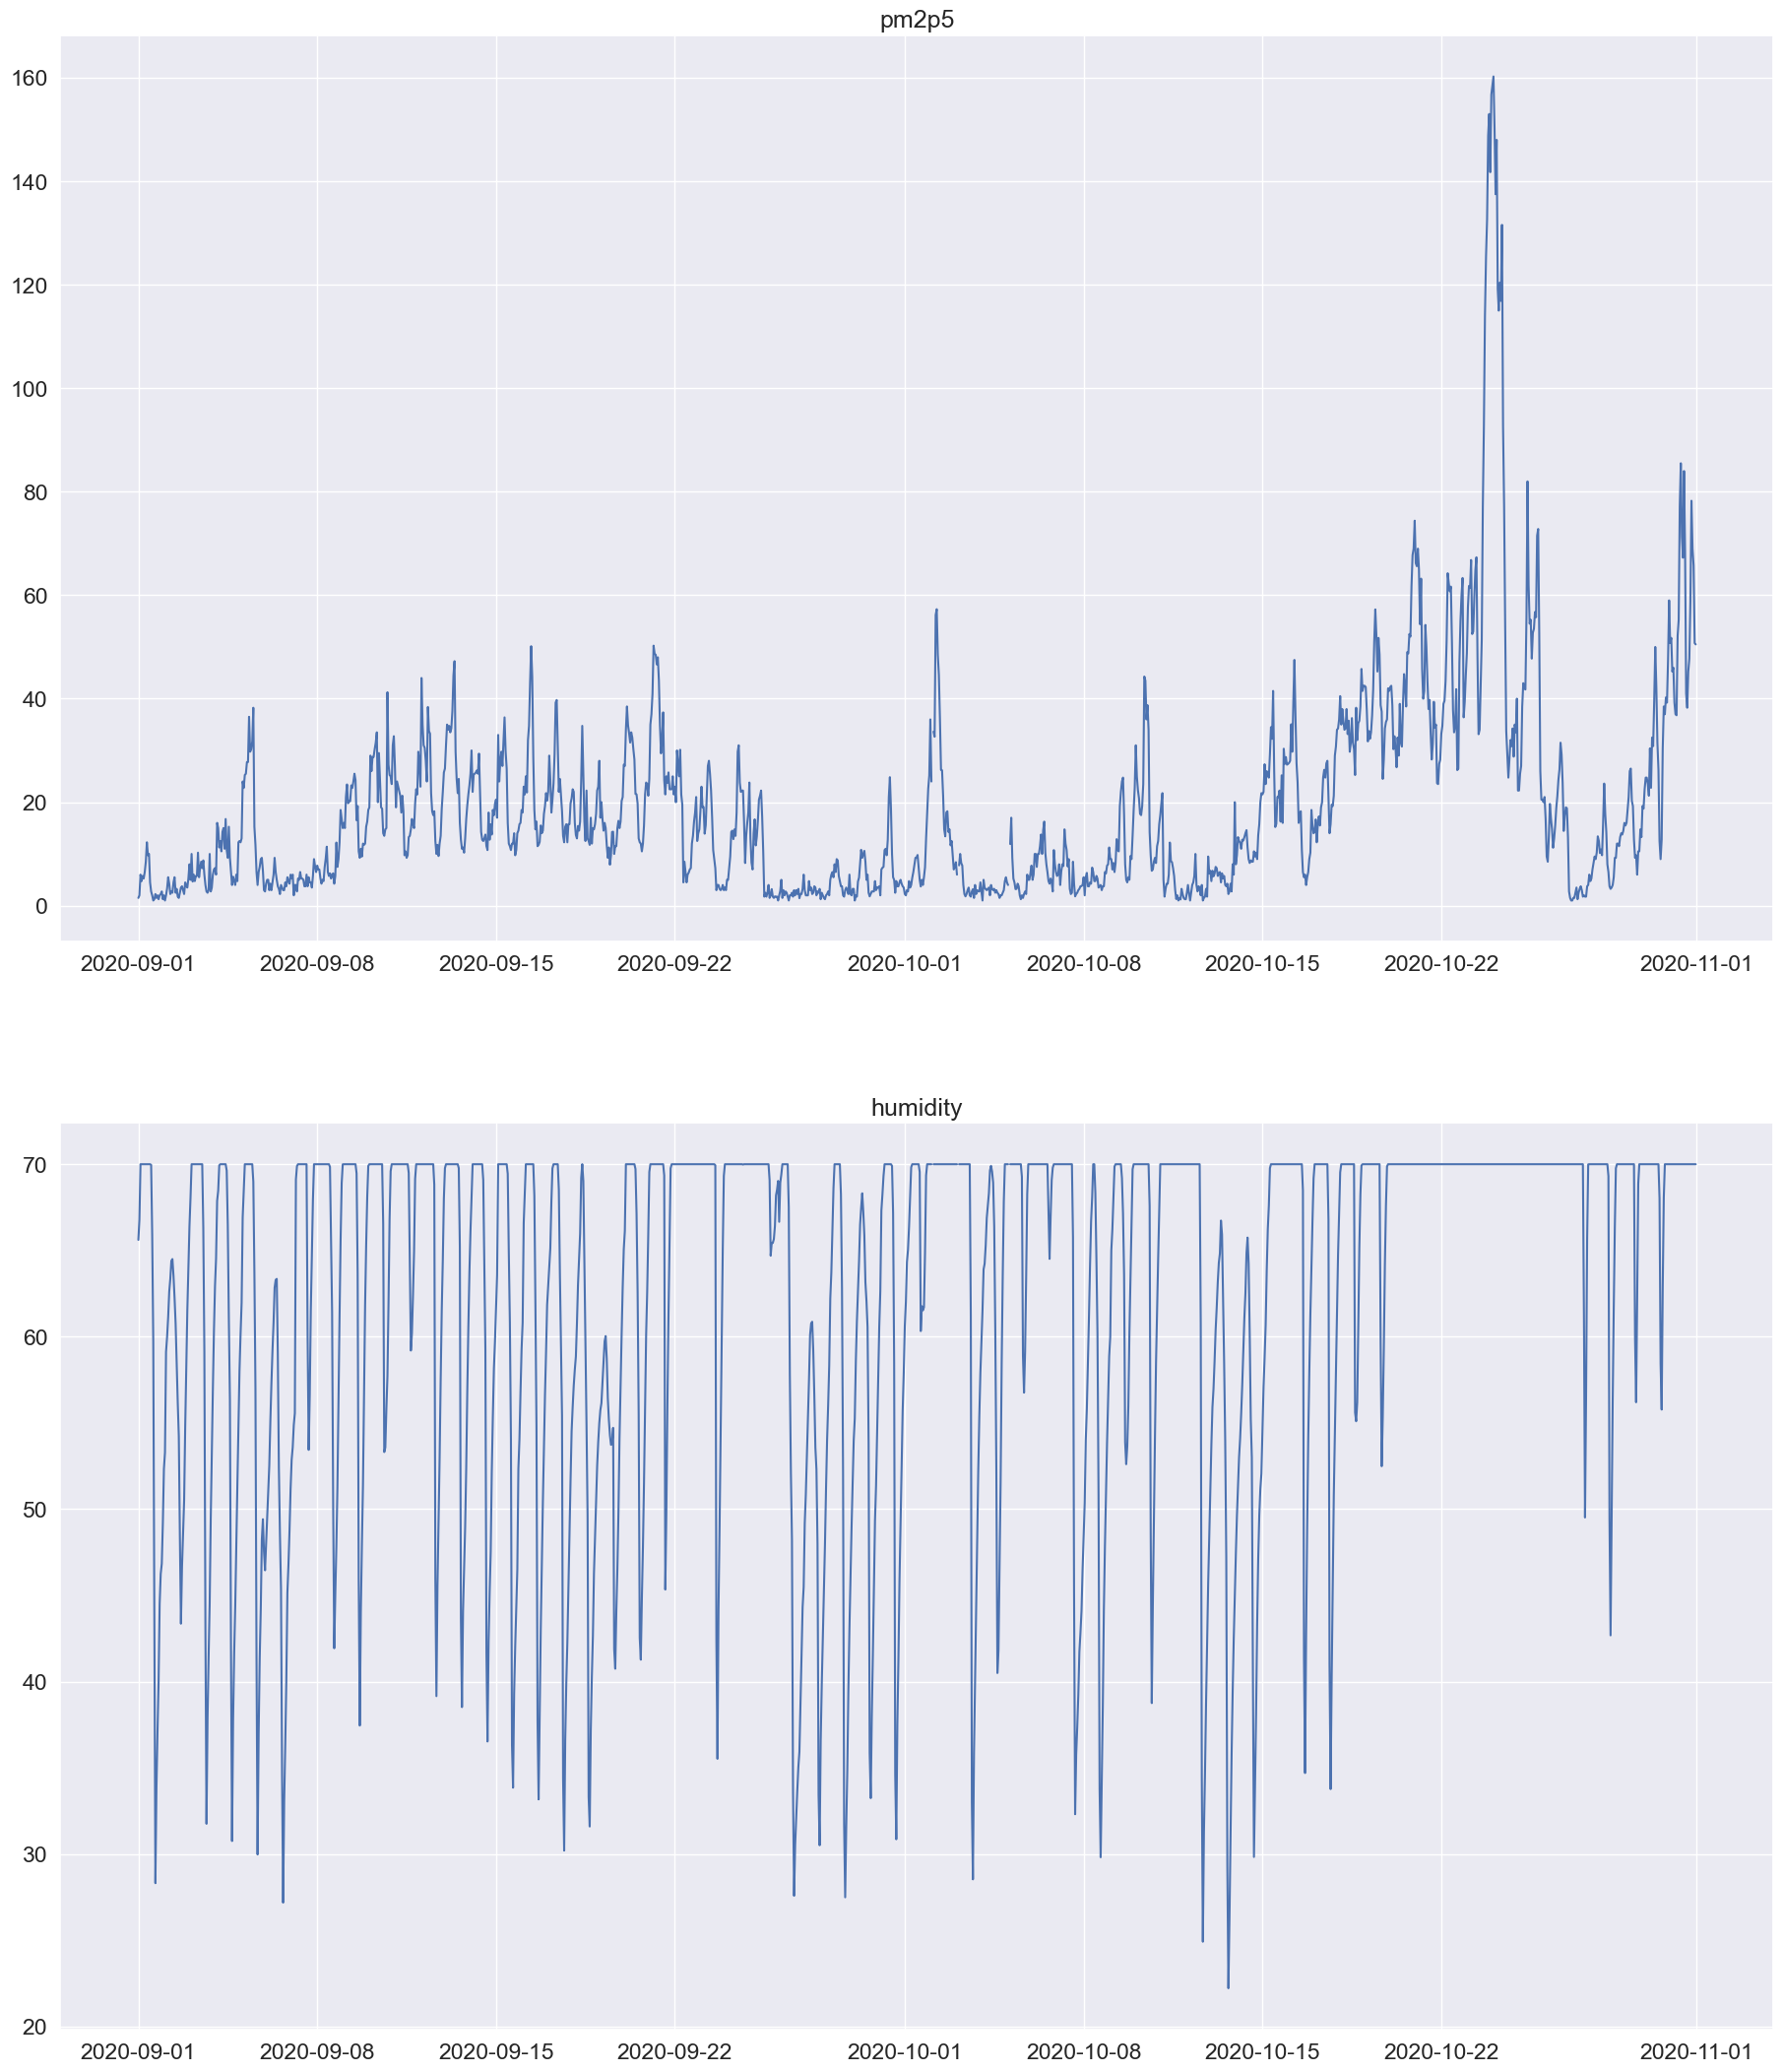
\includegraphics[scale=0.18]{humidityplot.png}
      \caption{(d) Plot of humidity vs pm2p5}
    \end{minipage}
  \end{figure}
The precision of sensors is negatively affected by special weather conditions (e.g.,
heavy rain, humidity, wind speed, temperature). Therefore, we examine atmospherical condition in order to find some interplay with the variation of pm2pm5.
 In the following graph, we show a qualitative comparison in the effect of rain, wind,humidity and temperature with the variation of pm2p5 in 48h for the potid 1091. 
 \\As for the moment just observe that there does not appear to be a strong relationship between
pm2p5 and rainy level or wind speed or temperature. A bit different is the nature of humidity. Even though the time series seems to
have a natural periodicity, the action of humidity sometimes disrupts this behaviour, since there is a big peak of pm2p5
in correspondence of a continuous high level of humidity(in the end of October).
\begin{wrapfigure}{r}{0.5\textwidth}
    \centering
    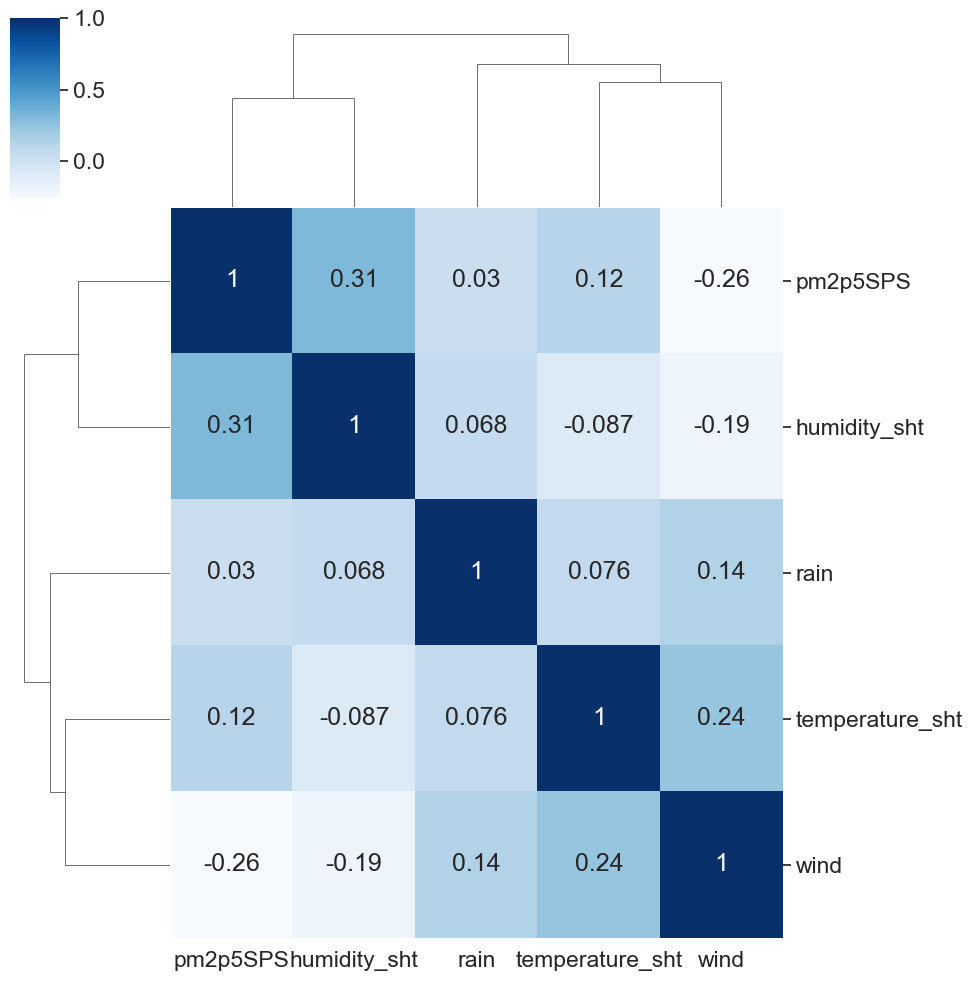
\includegraphics[scale=0.4]{correlations.png}
    \caption{clustermap}
\end{wrapfigure}

This can be seen also through the clustermap below, which plot a matrix dataset as a hierarchically-clustered heatmap . 
Motivated by these results, we will try to take into account this fact in our future analysis. 

\subsection{Stationarity}

In order to check the possibility to consider our model as a structural time series, we check the stationary of our time series such that its statistical properties (such as mean, variance, autocorrelation, etc.) are all constant over time. 
To check whether a series is stationary, we can apply the Augmented Dickey fuller test.
Since the p-value of the test is 0.020 we can reject the null hypothesis that the series is non-stationary. 

\section{Model}
Autoregressive time series models are central to stationary time series data analysis. Therefore, as  a first proposal, we choose an AR(2) model for the univariate case and we are going to extend this model with more complicated models for the multivariate case. We make this choice focusing on the analysis of the autocorrelation (ACF) and partial autocorrelation plot (PACF) of the pot 1091: 
since ACF tails off and PACF cuts off after one lag, then we are dealing with an AR(2) model (see figure~\ref{fig:acf} and~\ref{fig:pacf}).

  \begin{figure}[h!]
    \centering
    \begin{minipage}[t]{0.4\textwidth}
      \centering
      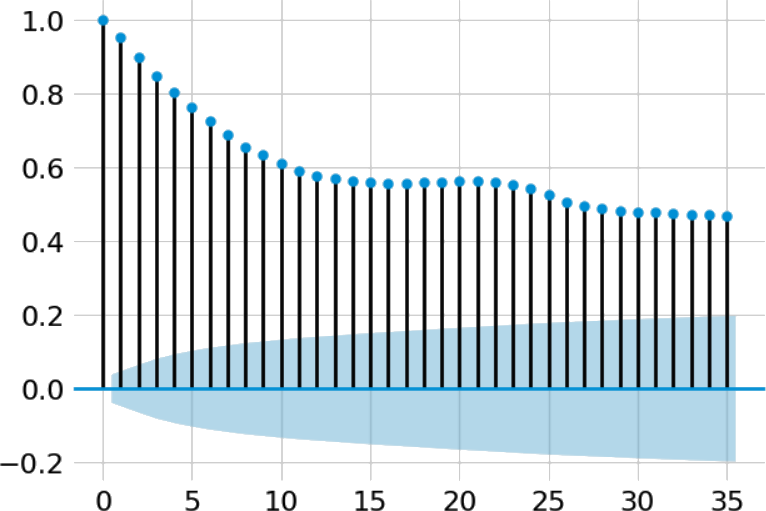
\includegraphics[scale=0.3]{acf.png}
      \caption{Autocorrelation plot for the 1091 pot series}\label{fig:acf}
    \end{minipage}\hfill
    \begin{minipage}[t]{0.4\textwidth}
      \centering
      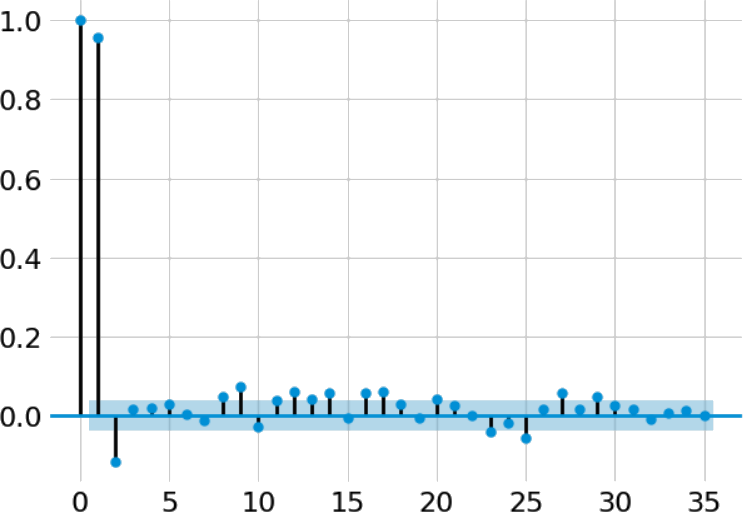
\includegraphics[scale=0.3]{pacf.png}
      \caption{Partial autocorrelation plot for the 1091 pot series}\label{fig:pacf}
    \end{minipage}
  \end{figure}

As a first proposal, we assume a conjugate model to explain the AR(2) structure of the time series:
\begin{equation*}
    y_t = \phi_1 y_{t-1} + \phi_2 y_{t-2} + \epsilon_{t} \qquad \qquad \epsilon_{t} \sim \mathcal{N}(0, \sigma^2) 
\end{equation*}
where $\epsilon_{t}$ is a sequence of uncorrelated error terms and the $\phi_i$ are constant parameters.

\vspace{3mm}

\begin{tabularx}{0.8\textwidth}{XX}
    { 
        \text{LIKELIHOOD}\newline\newline
        \[
        \begin{aligned} 
        y|\underline{\phi},\beta & \sim N(\underline{\phi}^{T}\beta,\sigma^{2})\\
        & \text{$\sigma^{2}$ not known}
        \end{aligned}
        \]
    }&{
        \text{PRIORS}\newline\newline
        \[
        \begin{aligned}
	    \underline{\phi }|\sigma^2 &\sim \mathcal{N}_2(\underline\mu_0, \sigma^2B_0) \\
        \sigma^2 &\sim inv\Gamma \Bigl(\frac{\nu_0}{2}, \frac{\nu_0 \sigma_0^2}{2} \Bigr) \qquad
        \text{with $\mu_0, B_0, \nu_0, \sigma_0^2$ fixed}
        \end{aligned}
        \]
	
    }
\end{tabularx}

\vspace{3mm}

$B_0$ is a $2 \times 2$ matrix, $\mu_0$ is any vector in $\mathcal{R}^2$. Because the model is a standard conjugate linear model, posteriors are:

\text{POSTERIORS}\newline\newline
\[
\begin{aligned}
\underline{\phi} | Y &\sim \mathcal{N}_2 (\mu_n, \sigma^2 B_n)
\qquad \qquad
\begin{aligned}
    & \mu_n = \mu_0 + B_0 \Phi[\Phi^{T} B_0 \Phi + I_n]^{-1}(Y - \Phi^T\mu_0) \\
    & B_n = B_0 - B_0\Phi[\Phi^{T} B_0 \Phi + I_n]^{-1}\Phi^T B_0 \\
\end{aligned} \\
\sigma^2 | Y &\sim inv\Gamma \Biggl(\frac{v_n}{2}, \frac{v_n \sigma_n^2}{2} \Biggr) 
\qquad \qquad 
\begin{aligned}
    & v_n = v_0 + n \\
    & \sigma_n^2 = \frac{1}{v_n} \Bigl[ v_0\sigma_0^2 + (Y - \Phi^T\mu_0)^T [\Phi^T B_0 \Phi + I_n]^{-1} (Y - \Phi^T\mu_0) \Bigr]
    \end{aligned}\\
\end{aligned}
\]
\vspace{10mm}

Unfortunately can happen that sensor does not send any data. From our perspective this translates in the presence of missing values in the time series. For this univariate analysis pot 1091 has only the 0.012\% of value missing, hence in this case is not a particular problem. Morover missing data are distributed over the all considered period (we have missing values in correspondence of just few hours) and do not span a large interval of time.

\end{document}
